\documentclass[10pt]{article}

\usepackage[utf8]{inputenc}

\usepackage{graphicx}
\usepackage{amsmath}
\usepackage{amssymb}
\usepackage{algorithm,algorithmic}
\usepackage{float}
\usepackage{caption}
\usepackage{cleveref}

\usepackage[citestyle=authoryear,natbib=true,backend=bibtex]{biblatex}
% \addbibresource{ressources.bib}
% \usepackage{natbib}
\bibliography{ressources.bib}


\newcommand{\sectionbreak}{\clearpage}



\renewcommand\vec[1]{\boldsymbol{\mathbf {#1}}}
\newcommand\R{\mathbb {R}}
\newcommand\doubleminipage[2]{
\begin{figure}[H]
\centering
\centerline{
\begin{minipage}{0.5\textwidth}
    \caption*{\footnotesize GTN trained with \texttt{'base\_larger'}}%
    \includegraphics[trim=10 0 0 30,clip,width=\textwidth]{figures/base_larger_#1.pdf}
\end{minipage}%
\begin{minipage}{0.5\textwidth}
    \caption*{\footnotesize GTN trained with \texttt{'base\_larger3'}}%
    \includegraphics[trim=0 0 10 30,clip,width=\textwidth]{figures/base_larger3_#1.pdf}
\end{minipage}
}
\caption{#2%
\label{fig:results_#1}
}
\end{figure}
}



\title{
Evaluating the Robustness of \\
Generative Teaching Networks \\[5pt]
% Accelerating Neural Architecture Search \\
% by Learning to Generate Synthetic Training Data \\[5pt]
\large{\textit{Felipe Petroski Such, Aditya Rawal, Joel Lehman, Kenneth O. Stanley, Jeff Clune}}}
\author{Kurt Willis}
\date{\today}
% \institute{TU Berlin}

\begin{document}

\maketitle

\begin{abstract}
    Training machine learning models from scratch is 
    computationally demanding 
    and efficient network training is desirable in order 
    to reduce cost and time demands.
    Generative Teaching Networks, a meta-learning algorithm, 
    have been proposed to rapidly train new architectures
    and can even be beneficial to Neural Architecture Search.
    This work is motivated by the question if possible downsides
    exist for training models in this fashion or if perhaps
    it comes with benefits by running robustness performance
    tests and comparing to traditionally trained models.
\end{abstract}

\section{Introduction}
\textit{Meta-learning} is concerned about "learning to learn". 
In machine learning there are generally 3 components that come into play.
The \textbf{environment}, the learner \textbf{model} and the learning \textbf{algorithm}.
In traditional machine learning, the environment and the algorithm are seen as fixed.
Only the model weights are adapted via the learning algorithm 
after receiving a signal from the environment (through the training data).
Generative Teaching Networks (GTNs) \citep{such2019generative} aim to learn the environment
and parameters of the learning algorithm to accelerate the learning process
for a variety of different kinds of models.
The environment and algorithm parameters are learned 
via meta-learning by maximizing the performance
of models trained via GTNs on the training data.


% \begin{figure}
%     \centering
%     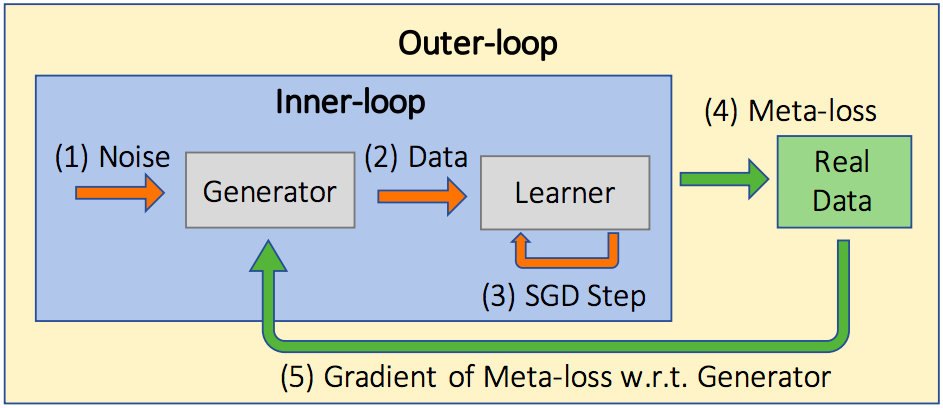
\includegraphics[width=\textwidth]{figures/Meta-Learning.png}
%     \caption{Generative Teaching Networs Outer-loop \cite{andrychowicz2016learning}}
%     % \label{fig:my_label}
% \end{figure}

A \textit{Generative Teaching Network} is a generative model
that is able to generate images from a latent vector $\vec z$
coming from some latent distribution. 
One outer-loop cycle (meta training step) 
consists of a full network training cycle
(64\footnote{The workings of GTNs will be illustrated by presenting the specific hyperparameter values used in the experiments, although most of these can be set arbitrarily.} inner-loop update steps).

\begin{algorithm}[H]
\caption*{\textbf{Algorithm} Generative Teaching Networks}
\begin{algorithmic}
\STATE initialize $G_{\vec\omega}$
\FOR{\texttt{2000 times}}
\STATE sample $D_{\vec\theta}$
\FOR{\texttt{64 times}}
    \STATE $\vec z = (\vec z_x, \vec z_y) \sim \text{sample randomly}$
    \STATE $\vec x \gets G_{\vec\omega}(\vec z)$
    \STATE $\hat {\vec y} \gets D_{\vec\theta}(\vec x)$
    \STATE ${\vec\theta} \gets {\vec\theta} - \lambda \nabla_{\vec\theta} \mathcal L(\hat{\vec y}, \vec z_y)$
\ENDFOR
\STATE ${\vec\omega} \gets {\vec\omega} - \gamma \nabla_{\vec\omega} \mathcal L(D_{\vec\theta}(\vec x_{\texttt{train}}), \vec y_{\texttt{train}})$
\ENDFOR
\end{algorithmic}
\end{algorithm}

\noindent
An inner-loop cycle consists of 
\begin{enumerate}
    \item Randomly sampling a latent vector 
          $\vec z = (\vec z_x, \vec z_y) \in \R^{128 + 10}$
          (consisting of a latent code $\vec z_x$ and a label $\vec z_y$).
    \item Generating an image $\vec x = G_{\vec \omega}(\vec z) \in \R^{28\times28}$
          by passing the latent vector $\vec z$ to the generator $G_{\vec \omega}$.
    \item  Calculating the class probability vector (predicted label) $\hat {\vec y} = D_{\vec \theta}(\vec x) \in \R^{10}$
    by passing the image $\vec x$ to the discriminator network $D_{\vec \theta}$.
    \item Updating the weights of the discriminator $D_{\vec \theta}$
    by evaluating the cross-entropy loss $\mathcal L(\hat {\vec y}, \vec z_y)$
    and computing the gradient with respect to $\theta$.
\end{enumerate}
The outer-loop performs the following steps.
\begin{enumerate}
    \item Sampling a new discriminator model $D_{\vec \theta}$ and randomly initializing it.
    \item Performing 64 inner-loop update steps on $D_{\vec \theta}$.
    \item Updating the weights of the generator $G_{\vec \omega}$
    by evaluating the final performance of $D_{\vec \theta}$ 
    on the training set $(\vec x_\texttt{train}, \vec y_\texttt{train})$
    and computing the gradient with respect to $\omega$.
\end{enumerate}
% $\frac {\partial \mathcal L(D_\gamma(G_(\vec z_x)), \vec z_y)} {\partial \gamma}$.
The signal obtained by evaluating the discriminator on the training set is back-propagated 
through all of the 64 inner update cycles.
This signal can also be used to learn further differentiable hyperparameters, 
such as the optimizer learning rate.
All quantities, ($\vec z$, $\vec x$, \ldots) are batched in
mini-batches of size $128$.

In the main setup: \textit{full curriculum}, the latent vectors $\vec z$,
the learning rates and momentum parameters are learned for each of
the 64 update steps.
When dealing with the MNIST dataset this can result in over 95\%
accuracy after a few update steps.
By contrast, traditional, unoptimized "vanilla" learning
takes about 390 update steps to reach similar accuracies.

Although meta-learning itself comes with a lot of overhead, 
working with a trained GTN comes with a few benefits.
The authors mention rapid training and efficient Nerual Architecture Search \cite{such2019generative}.
This work will further examine trade-offs by running 
robustness performance tests for models trained with GTNs
and these to models trained in a traditional manner.

However, first some general notes.
Training custom architectures with a trained GTN did not work out of the box. 
The possible architecture choices are limited. For example, weight normalization is required and batch normalization does not work. The authors make note of this, however, pooling layers also don't seem to work.
This means the tests are restricted to a small set of selected architectures.
The authors seem to train the GTN on one fixed architecture only. The rate of success of transferring a trained GTN to another architecture is limited.


\section{Robustness Performance Tests}

The following performance tests only focus on the MNIST dataset, as the 
CIFAR10 dataset results were deemed too unreliable to make any significant claims.
For all experiments, two different GTN models have been trained that were optimized for the \texttt{'base\_larger'} and \texttt{'base\_larger3'} models respectively.
These two GTN choices each trained a total of 9 different architecture \textit{learner types}.
Furthermore, three different learning algorithms are considered, \texttt{'10\_gtn'}, \texttt{'gtn'} and \texttt{'vanilla'}.
Models trained with \texttt{'10\_gtn'} received 10 (inner loop) update steps from the GTN, \texttt{'gtn'} the full 64 steps.
Models trained with \texttt{'vanilla'} are trained with a classical learning algorithm (Adam optimizer, 1 epoch over training data).
In order to have a fair comparison, the criteria for accepting models of a certain learner type is that the minimum value over the learning algorithms (\texttt{'10\_gtn'}, \texttt{'gtn'}, \texttt{'vanilla'}) has a mean accuracy greater than 0.7 for 5 individually trained models.
This limited the choice of available learner types to only two (\texttt{'base\_larger'} and \textit{'base\_larger3'}) of 9.

The robustness tests include input corruption by augmentation
(adding noise and blurring) and the FGSM and LBFGS adversarial attacks.
All tests are performed on unseen test data of size 10,000 and 1,000
for the augmentation and adversarial attacks respectively.
In all tests, the input image is clipped to its valid range.

\subsection{Noise Corruption}

In this setting, Gaussian noise that is sampled from a normal distribution
with standard deviation of $\beta$ is added to the input.

$$
\tilde {\vec x} = \text{clip}[\,\vec x + \beta \vec z\,] \,, \quad \vec z \sim \mathcal N(\vec 0, \vec I)
$$

\begin{figure}[H]
    \centering
    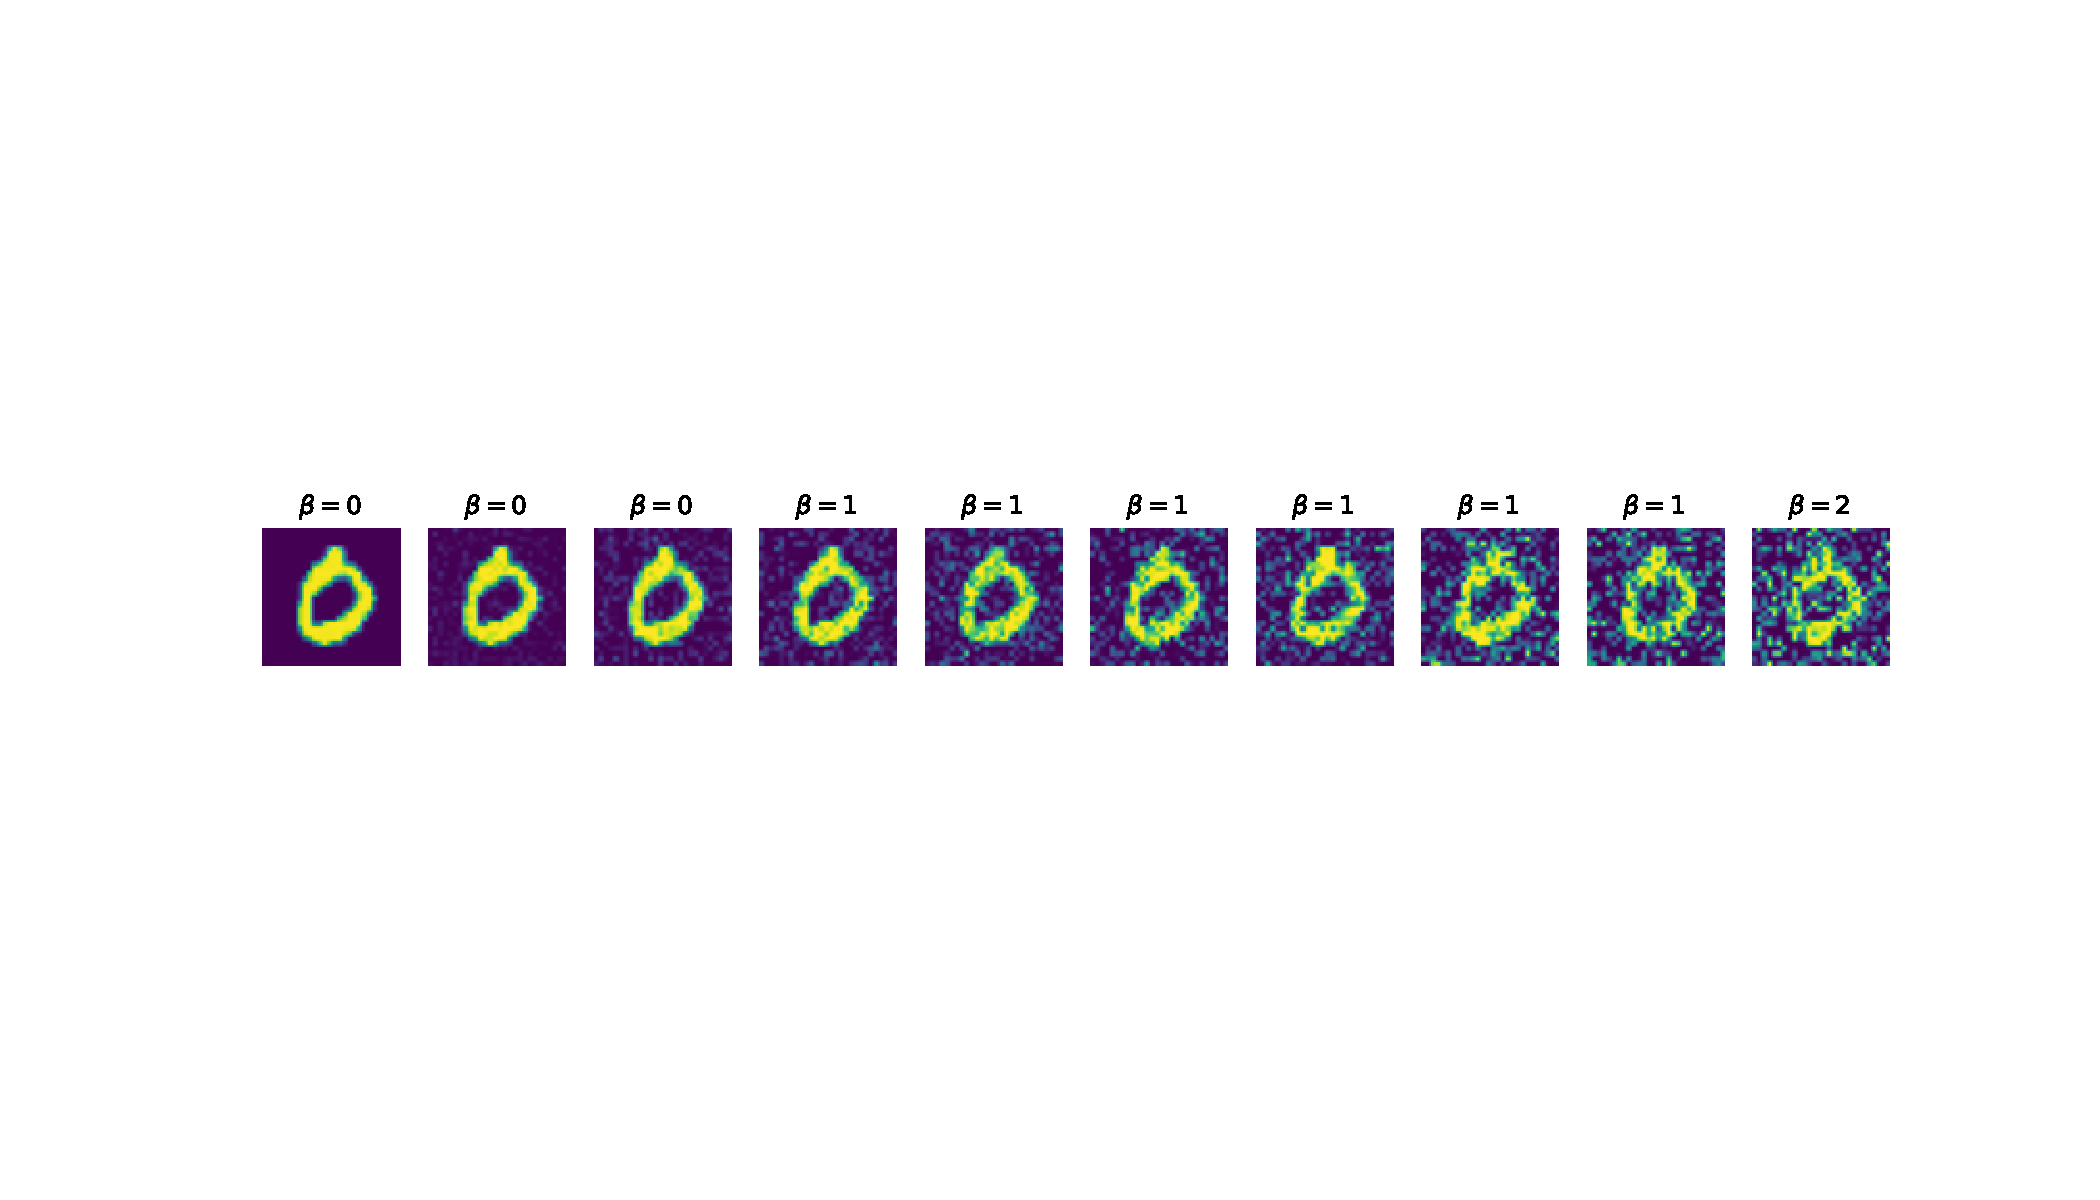
\includegraphics[trim=200 250 100 200, clip, width=\textwidth]{figures/samples_noise.pdf}
    \caption{Noise corruption of varying strength $\beta$.}
    \label{fig:samples_noise}
\end{figure}

\Cref{fig:samples_noise} shows a randomly selected input example with varying
noise strengths.

\doubleminipage{noise}{Accuracies of trained models under varying input noise corruption.}

\Cref{fig:results_noise} shows the results of the noise corruption performance tests.

\subsection{Blurring}
For this test, 
a blur filter is applied to the input via convolution with a Gaussian kernel
with standard deviation of $\beta$.

$$
\tilde {\vec x} = \text{gaussian\_blur} _\beta (\vec x)
$$

\begin{figure}[H]
    \centering
    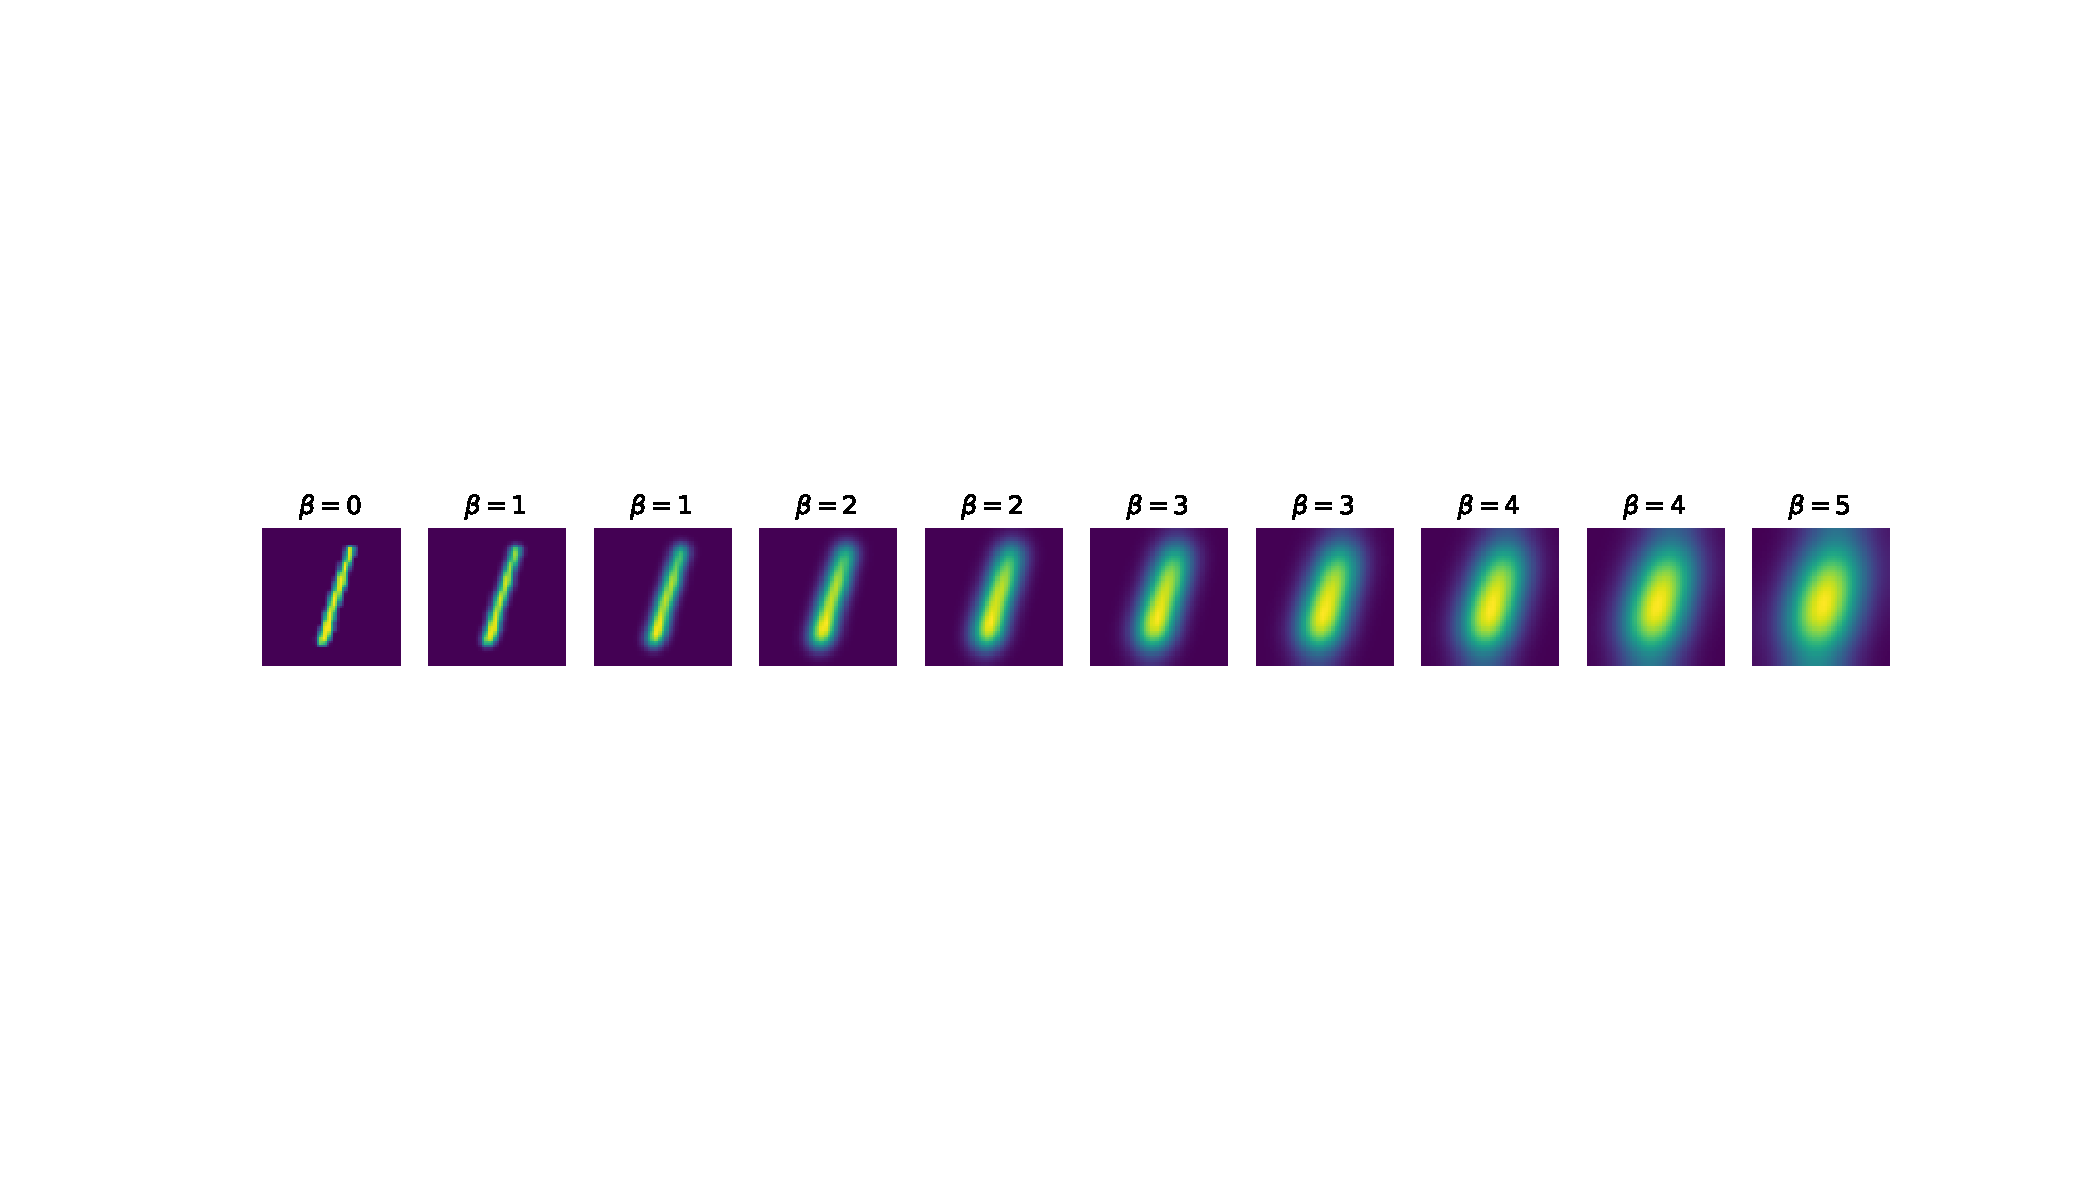
\includegraphics[trim=200 250 100 200, clip, width=\textwidth]{figures/samples_blur.pdf}
    \caption{Gaussian-blur filter applied with varying Gaussian kernel std $\beta$.}
    \label{fig:samples_blur}
\end{figure}


\doubleminipage{blur}{Accuracies of trained models under varying Gaussian-blur filters.}

\subsection{FGSM-Attack}
The Fast-Gradient-Sign-Method is performed by calculating
the gradient of the loss with respect to the input.
The input is then moved by $\beta$ in the direction (sign)
of increasing loss. This is done for $30$ steps. 
The formula for the update step is given in \cref{eq:fgsm}.
\Cref{fig:samples_fgsm} shows the outcome of varying $\beta$ strengths on
a random sample.

\begin{align}
\label{eq:fgsm}
\begin{split}
\vec x &\gets \vec x + \beta \, \text{sign}\left(\nabla_{\vec x} \mathcal L(D(\vec x), y)\right) \\
\vec x &\gets \text{clip}[\, \vec x \,]
\end{split}
\end{align}
%
\begin{figure}[H]
    \centering
    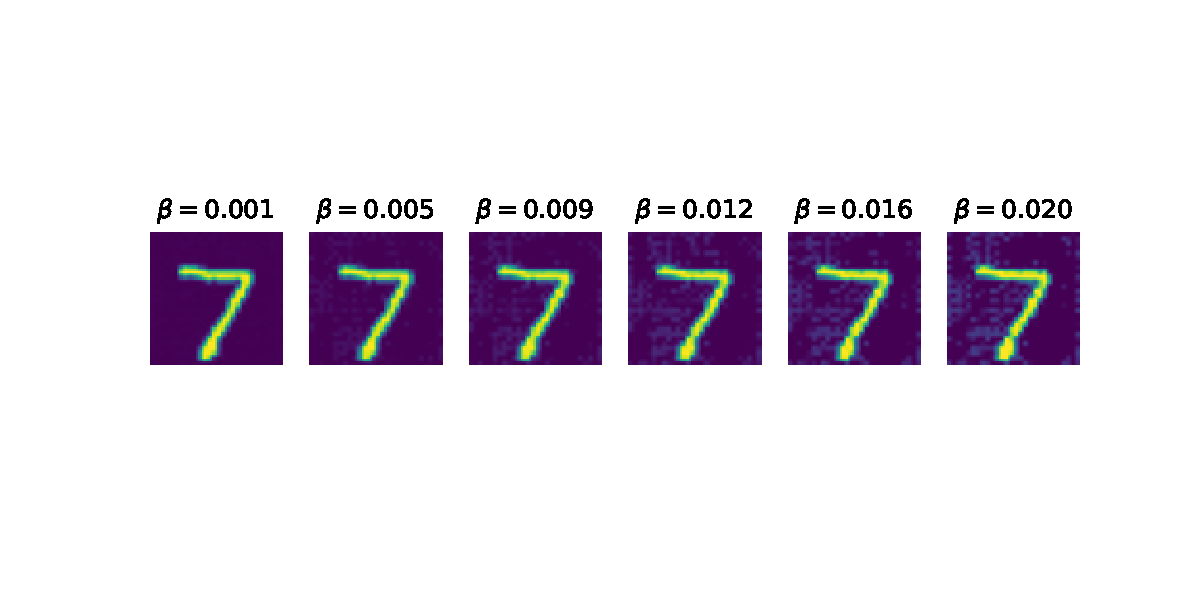
\includegraphics[trim=0 100 0 80, clip, width=0.8\textwidth]{figures/samples_fgsm.pdf}
    \caption{Results after 30 steps of FGSM-attack with varying $\beta$.}
    \label{fig:samples_fgsm}
\end{figure}
\doubleminipage{fgsm}{Accuracies of trained models under FGSM-attack with varying strengths.}

\subsection{LBFGS}
The Box-constrained LBFGS-attack is performed similarly to the FGSM-attack 
by calculating
the gradient of the loss with respect to the input.
The loss here, however, is the cross-entropy loss minus the $l2$ distance
of the current input to the original input multiplied by $\frac 1 \beta$
(this ensures that the computed adversarial output stays close to
the original sample).
The input is then moved by the update rate $\varepsilon=0.002$ times the gradient of the loss. 
This is also done for $30$ steps. 
The formula for the update step is given in \cref{eq:fgsm}.
\Cref{fig:samples_lbfgs} shows the outcome of varying $\beta$ strengths on
a random sample.

\begin{align}
\label{eq:lbfgs}
\begin{split}
\vec x &\gets \vec x + \varepsilon \left( \nabla_{\vec x} \mathcal L(D(\vec x), y)
- \frac 1 \beta \nabla_{\vec x} \| \vec x - \vec x^0 \|_2 \right) \\
\vec x &\gets \text{clip}[\, \vec x \,]
\end{split}
\end{align}

\begin{figure}[H]
    \centering
    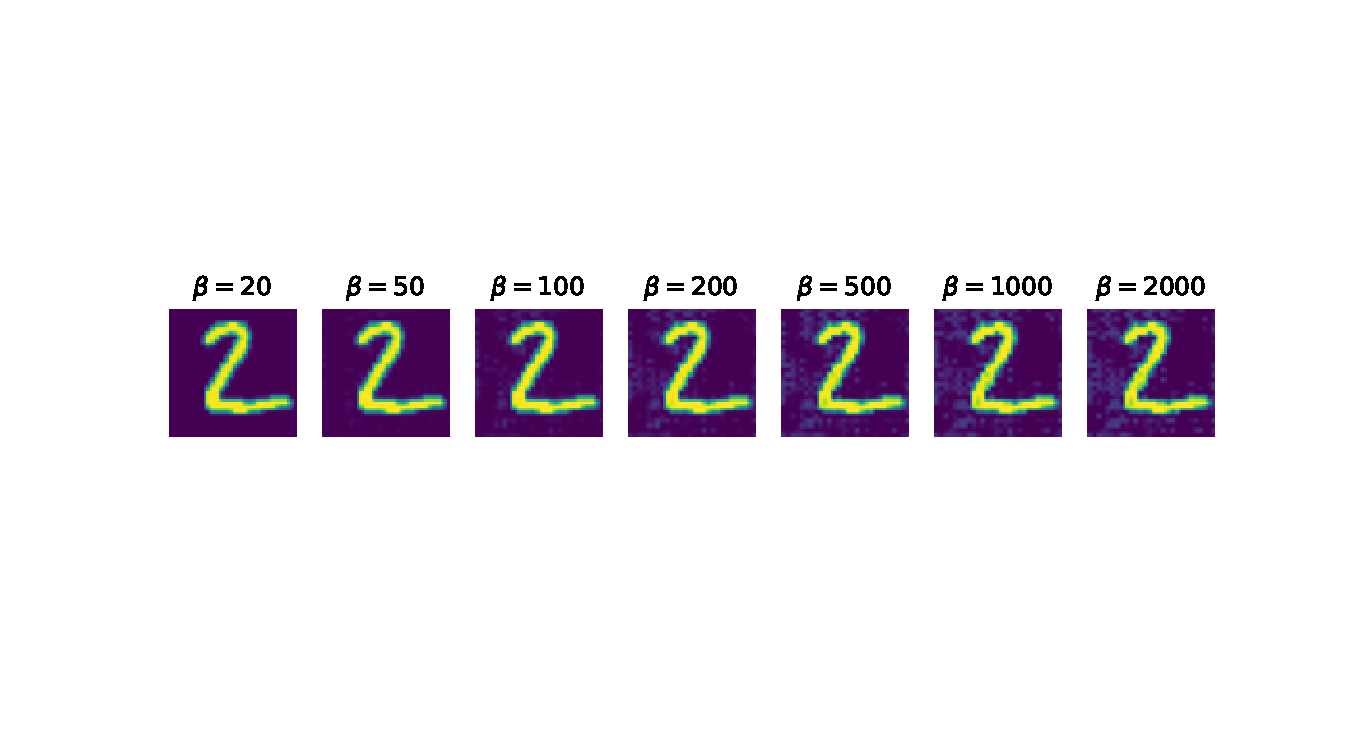
\includegraphics[trim=0 150 0 100, clip, width=\textwidth]{figures/samples_lbfgs.pdf}
    \caption{Results after 30 steps of LBFGS-attack with varying $\beta$.}
    \label{fig:samples_lbfgs}
\end{figure}


\doubleminipage{lbfgs}{Accuracies of trained models under LBFGS-attack with varying strengths.}


\section{Conclusion}

The general narrative has been that training a network to higher accuracies
leads to decreasing generalization \citep{zhang2019theoretically}. This is verified by comparing
the networks trained with GTNs for the full 64 steps with those 
trained for only 10 steps.
However, networks trained with a vanilla learning algorithm
seem to, for the most part, outperform those trained by GTNs
while still showing increased robustness towards input corruption and 
adversarial attacks.
This leads to the conclusion that networks trained with GTNs 
are indeed less robust compared to those trained in a traditional way.
However, since these experiments are only run on one dataset and GTNs will likely improve over time, more data is required to make any substantial claims.

\appendix

\printbibliography

\end{document}